\chapter{Anhang 1}
\label{chap:appendix1}
% -------------------------------------------------------------

\section{Alternative Figure GCC}
\label{appendix:a1_alternativeGcc}

Figure of \ac{GCC} with filters before the correlation.
\change[]{Better description?}
\begin{figure}[ht]
	\centering
		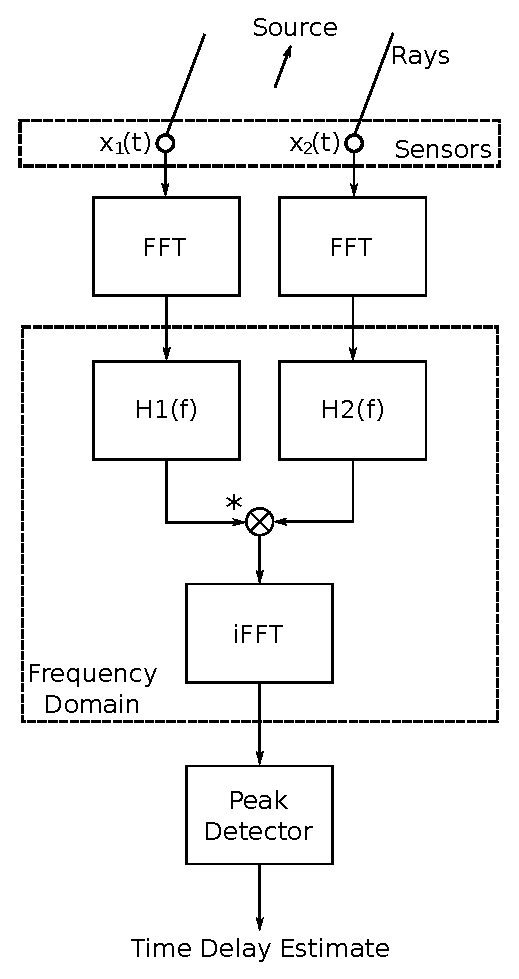
\includegraphics[width=0.35\columnwidth]{figures/GCC}
	\caption{Generalized cross correlation for time delay estimation.}
	\label{fig:ap1_GCC}
\end{figure}
% -------------------------------------------------------------

\section{GCC Method Frame Shift}
\label{appendix:a1_gccFrameShift}

Link between \ac{PSNR} and correctness of the whistle-source direction
detection on one robot is charted.
Data of all measurements of \cref{subsec:04_labMeasurements} on robot 26
are used.

\begin{figure}[ht]
	\centering
		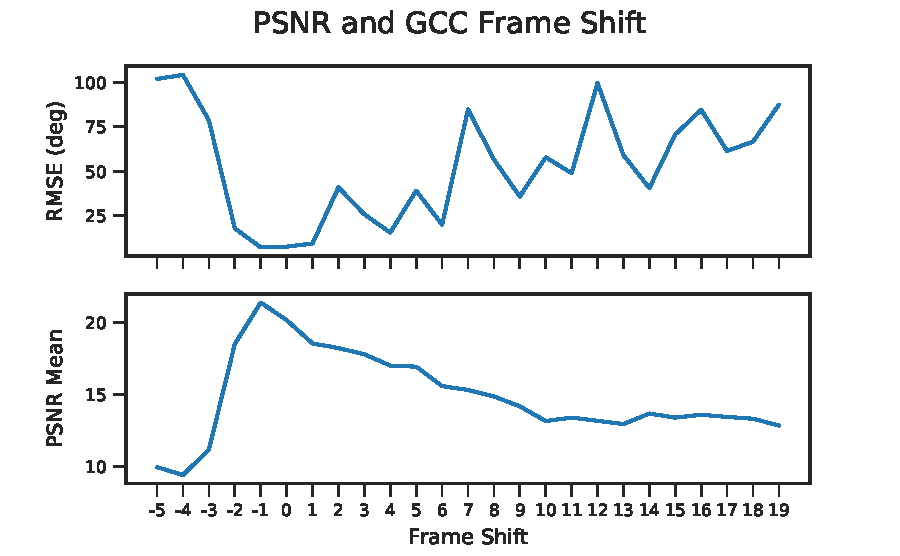
\includegraphics[]{figures/evaluation/psnr_frame_shift_all_measurements}
	\caption{Frame window shifted around start index. All measurements of
	\cref{subsec:04_labMeasurements} are utilized for robot at center point. }
	\label{fig:ap1_gccFrameShiftAllMeasurements}
\end{figure}
% -------------------------------------------------------------